\chapter{Holographic Video Microscopy}
\label{ch:hvm}

% Suggested figures.
% Diagrams depicting the physical processes
% sequentially.
% The setup.

\newcommand{\einc}{\vec{E}_{\text{inc}}}
\newcommand{\escat}{\vec{E}_{\text{s}}}
\newcommand{\eadd}{\vec{E}_{\text{add}}}

\section{Overview}

%In this chapter, we will review the salient details 
%underlying the theory and experimental implementation
%of holographic video microscopy. Whenever possible,
%extraneous details that detract from our narrative
%will be relegated to the appendix or be given 
%primary source citations.


%Holographic video microscopy illuminates a sample of scatterers with
%coherent illumination in order to preserve phase information.
Holographic video microscopy (HVM) utilizes coherent
illumination to measure properties of micron-sized particles,
primarily their size, refractive index, and three-dimensional position.
By imaging a sample with coherent illumination, the normally averaged-away
phase information is preserved and contributes to the intensity variations
in the resulting image. The physical properties of individual scatterers
are encoded in this phase information and can be extracted by fitting
the resulting intensity patterns to an appropriate light scattering theory.
For non-absorbing dielectric spheres between $\num{1}$-$\SI{10}{\um}$,
this technique yields nanometer-scale precision for the three-dimensional
position and radius, and part-per-thousand precision for the refractive index.

In this chapter, we acquaint the reader with our primary experimental
HVM setup and in so doing outline the salient physical processes underlying
the technique. We then describe the Lorenz-Mie theory of light
scattering, % and discuss the validity of common assumptions.
discuss our implementation of image analysis, and 
conclude with a number of applications of holographic video
microscopy.


\section{Experimental Setup}
\label{ch:hvm:sec:hvm}

A diagram of our custom-built in-line holographic microscope
is provided in Fig.~%\ref{fig:hvm_01}.
Our setup illuminates
the sample plane with a blue ($\SI{447}{nm}$ vacuum wavelength),
linearly polarized laser beam (Coherent Cube). The beam's
$\SI{25}{\mW}$ of power is spread over the $\SI{3}{\mm}$ beam
diameter, producing an average irradiance of approximately
$\SI{0.88}{\mW / \mm^2}$. Before scattering through the
sample, the beam passes through a quarter-wave plate and a
polarizing beam splitter (ThorLabs CCM1-PBS251) to enable
beam attenuation and to optionally provide bright-field
illumination.

The coherent illumination and scattered light are collected by a
standard microscope objective (Nikon Plan Apo, $\num{100}$x,
numerical aperture $\num{1.45}$, oil immersion) and then focused
by a $\SI{200}{\mm}$ lens onto a greyscale digital camera
(NEC TI-324AII). The digital camera digitizes the resulting intensity
pattern to $8$-bits per pixel at $\SI{29.97}{frames / \sec}$ and relays the
resulting array of information to either a DVR (Pioneer 520HS) to record
on a DVD or directly to the hard disk of a personal computer.
Each pixel in the $\si{640 x 480}$ array of pixels has a width of
$\SI{13.5}{\um}$. After $100$x magnification, a pixel in the
image has an effective size of $\SI{0.135}{\um}$.

Each recorded image documents the interference between the incident
electric field and the resulting scattered waves. By fitting
to a theory of light scattering, we will measure the physical
properties of the scatterers contributing to the scattered fields
at the focal plane of the objective.

% Description of trapping?


  % BLURB connecting HVM to DHM
%Holographic video microscopy is one of several
%digital holographic microscopy (DHM) techniques.
%DHM differs from traditional bright-field microscopy
%by preserving, collecting, and making quantitative use of phase
%information. In most variants of DHM, each recorded
%wavefront can be numerically reconstructed, or rather
%{\it un}-propagated, all the way back to a scattering event
%to produce an image of the scatterer. By reconstructing
%several planes around the scatterer, each hologram
%can provide insight into the topography of each scatter
%in the field of view.

%Holographic video microscopy differs from DHM by analytically
%fitting the scatter's properties to the resulting

\begin{figure}
  \centering
  \includegraphics[width=\textwidth]{hvm_image_formation}
  \caption{A time series depicting the image formation process. (a) the incident
    electric field propagates in the $+\hat{z}$ direction. (b) the
    incident field passes through a spherical scatterer causing a
    spherically expanding scattered wave in response. (c) the incident
    field and the scattered field combine at the focal plane to produce
    an image.}
  \label{fig:image_formation}
\end{figure}


\subsection{Image formation}
\label{ch:hvm:sec:hvm:ssec:overview}

The image formation process at the focal plane of the objective
is depicted in Fig.~\ref{fig:image_formation}. Fig.~\ref{fig:image_formation}(a)
shows the coherent illumination, or incident field $\einc$, propagating in the $+\hat{z}$ direction
through the sample and toward the focal plane of the objective. We model the incident field
as a plane wave polarized in the $\hat{x}$ direction, 
\begin{equation}
  \label{eq:incidentfield}
  \einc(\vec{r}) = E_0\,  e^{i \varphi_0(\vec{r})} \, e^{i kz} \, \hat{x},
\end{equation}
with magnitude $E_0$, phase $\varphi_0$, and wavenumber
$k =\frac{2\pi n_m}{\lambda}$. All of the waves considered here
propagate with a time dependence of $e^{i \omega t}$. However,
our measurements of intensity will be time averaged over the course of an exposure period
of at least $\SI{10}{\us}$. As we will be imaging with $\SI{447}{nm}$ blue
light ($\omega \approx \SI{670}{THz}$), our time average will include
nearly \num{7} billion full cycles. We will therefore safely suppress the time
dependence in all of our waves.

As the incident illumination propagates freely through the sample, scatterers
with a refractive index mismatch with the medium will emit a diverging scattered wave,
$\escat$, in response. Fig.~\ref{fig:image_formation}(b) depicts the incident
field and resulting scattered field propagating toward the focal plane.
For the scatterers of interest in this study, the scattered field is dominated by
forward scattering and the scatterer will absorb a negligible amount of the
incident wave.


The incident field and scattered field continue propagating and eventually pass through
the focal plane, as depicted in Fig.~\ref{fig:image_formation}. The intensity of the image
formed in the focal plane can be described as
\newcommand{\preint}{\frac{n_mc\epsilon_0}{2}}
\begin{align}
  I &= \preint\abs{\einc + \escat}^2\\
    &= \preint\left ( \abs{\einc}^2 + \einc\cdot\escat^* + \einc^*\cdot\escat + \abs{\escat}^2 \right ) \\
    &= \preint\left (\abs{\einc}^2 + 2\Re\left \{\einc\cdot\escat^*\right \} + \abs{\escat}^2 \right ) \label{eq:image_formation}
\end{align}
where $n_m$ is the refractive index of the medium, $c$ is the speed of light in a vacuum,
$\epsilon_0$ is the vacuum permittivity, and we've assumed medium is non-magnetic
($\mu_r=1$).

The relative contributions of the terms in Eq.~\ref{eq:image_formation}
are depicted in Fig.~\ref{fig:three_contributions} for a $\SI{1.0}{\um}$ polystyrene
sphere ($n = 1.59$) a distance of $\SI{12}{\um}$ above an imaging plane with pixel
size $\SI{0.135}{\um}$.
The first term $\abs{\einc}^2$ is constant over the field of view and
incorporates no phase information. The third term 
$\abs{\escat}^2$ is also phase-less but is not constant over the field of view.
The second term, $2\Re\left \{\einc\cdot\escat^*\right \}$, contributes the
spatially-varying interference pattern from the relative phase of the incident
beam and the scattered wave and the intensity variations of the scattered wave.
% Discussion of DC terms? Does DC Stand for duty cycle?
% Pull out E_0?
% Discuss relative sizes of terms.



\begin{figure}
  \centering
  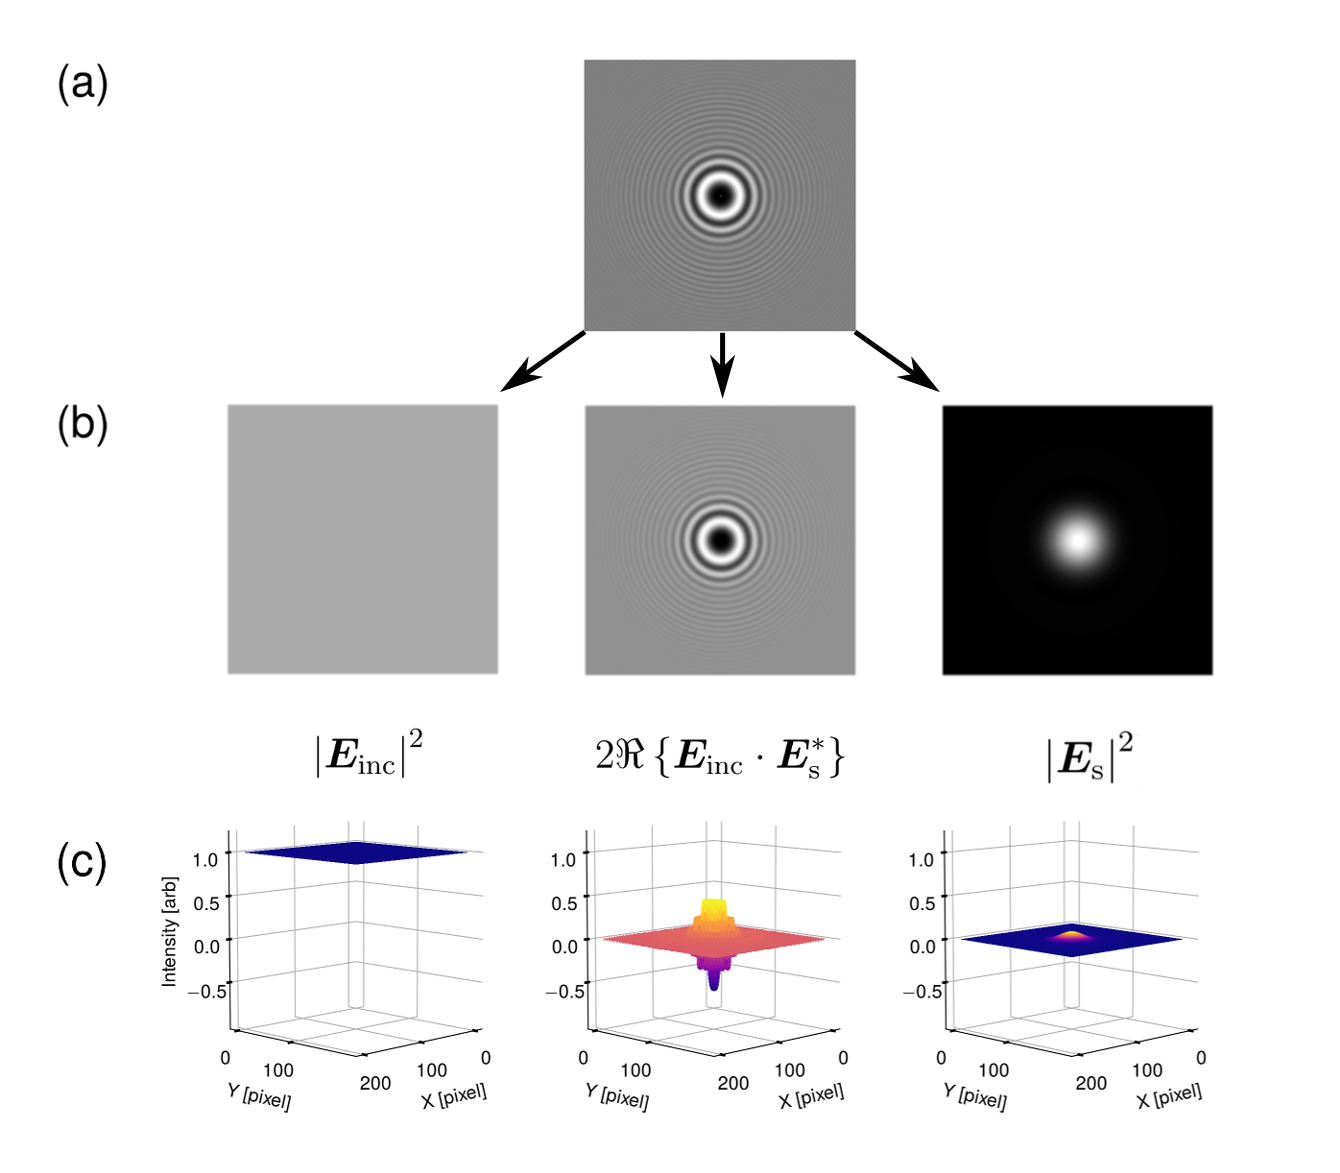
\includegraphics[width=\textwidth]{hvm_three_contributions}
  \caption{Depicting the three contributions to a holographic image. (a) the
    resulting intensity from a micron-sized scatterer above the focal plane.
    (b) The three contributions shown separately. (c) the magnitude of intensity
  for each term normalized by the intensity of the incident field.}
  \label{fig:three_contributions}
\end{figure}


\subsection{Scattering}
\label{ch:hvm:sec:hvm:ssec:scattering}

It is a general principle of linear, homogeneous media that the magnitude of the
scattered wave be proportional to the magnitude of the illuminating wave.
We therefore model the scattered field as

\begin{equation}
  \label{eq:incidentfield}
  \escat(\vec{r}) = E_0(\vec{r_p})\, \vec{f_s} \left ( k \left ( \vec{r} - \vec{r_p} \right ) \right ) ,
\end{equation}
where $E_0(\vec{r_p})$ is the average intensity illuminating the scatterer at $\vec{r_p}$,
and $\vec{f_s}$ describes how the particle $s$ scatters $\hat{x}$-polarized light.
Note that nature of $\vec{f_s}$ depends heavily on the shape and composition
of the scatterer.

%FIXME: Add rift about the spherical scatterer being parameterized by a_p, n_p, x, y, z

With the exception of \autoref{ch:dimpled}, our study will focus exclusively on
spherical scatterers. The Lorenz-Mie theory offers an exact solution for
the case of a spherical scatterer illuminated with $\hat{x}$-polarized light.
We will provide a minimalist account of the Lorenz-Mie theory to provide intuition
for the scattered wave's dependence on the spherical scatters properties; a thorough
account is provided in reference %FIXME: Add reference to Bohren.

\subsubsection{Lorenz-Mie Theory}
\label{ch:hvm:sec:hvm:ssec:scattering:sssec:lm_theory}




%The Lorenz-Mie theory
%constitutes an exact solution for a plane wave scattering off of a
%dielectric sphere in a homogeneous medium.

\begin{equation}
\label{eq:scatteredfield}
  \vec{f}_s(k \vec{r}) = \sum_{n=1}^\infty \, f_n \, \left(
    i a_n \, \vec{N}^{(3)}_{e1n}(k \vec{r}) - b_n \,
    \vec{M}^{(3)}_{o1n}(k \vec{r})
    \right),
\end{equation}
where $f_n=i^n (2n+1)/[n(n+1)]$, and $\vec{M}^{(3)}_{o1n}(\vec{x})$ and 
$\vec{N}^{(3)}_{e1n}(\vec{x})$ are the vector spherical harmonics,x
\begin{equation}
    \vec{M}^{(3)}_{o1n}(\vec{x}) = \frac{\cos\phi}{\sin\theta} \,
  P^1_n(\cos\theta) \, j_n(x) \, \uvec{\theta}
  - \sin\phi \, \frac{dP^1_n(\cos\theta)}{d\theta} \, j_n(x) \, \uvec{\phi},
\end{equation}
and
\begin{multline}
  \vec{N}^{(3)}_{e1n}(\vec{x}) = n(n+1) \, \cos\phi
  \,P^1_n(\cos\theta) \, \frac{j_n(x)}{x} \, \uvec{r} \\
  + \cos\phi \, \frac{dP^1_n(\cos\theta)}{d\theta} \,
  \frac{1}{x} \frac{d}{dx}\left[x j_n(x)\right] \, \uvec{\theta} \\
  - \frac{\sin\phi}{\sin\theta} \, P^1_n(\cos\theta) \,
  \frac{1}{x}\frac{d}{dx}\left[x j_n(x)\right] \, \uvec{\phi}
\end{multline}
Here, $P^1_n(\cos\theta)$ is the associated Legendre polynomial of the
first kind, and $j_n(kr)$ is the spherical Bessel function of the
first kind of order $n$.
The expansion coefficients in Eq.~(\ref{eq:scatteredfield}) are given
by \cite{bohren83}
\begin{equation}
  a_n = \frac{m^2 j_n(mka_p) \left[ka_p \, j_n(ka_p)\right]^\prime -
    j_n(ka_p) \left[mka_p \, j_n(mka)\right]^\prime}{
    m^2 j_n(mka_p) \left[ka_p \, h^{(1)}_n(ka_p)\right]^\prime -
    h^{(1)}_n(ka_p) \left[mka_p \, j_n(mka_p)\right]^\prime},
\end{equation}
and
\begin{equation}
\label{eq:bn}
  b_n = \frac{j_n(mka_p) \left[ka_p \, j_n(ka_p)\right]^\prime -
    j_n(ka_p) \left[mka_p \, j_n(m ka_p)\right]^\prime}{
    j_n(mka_p) \left[ka_p \, h^{(1)}_n(ka_p)\right]^\prime -
    h^{(1)}_n(ka_p) \left[mka_p \, j_n(mka_p)\right]^\prime},
\end{equation}


% Note that the inplane position of the image 

\subsection{Image Analysis}

We analyze each of our recorded images to extract information about the particles
scattering light into the field of view.  Because the scattered wave's electric
field approximately decays as $~\frac{1}{r}$, each scatterer's influence on the
resulting image can effectively be isolated to a sub-region of the image; we will
regard each of these sub-regions as holographic features.  Given an experimental
image, our task will be to isolate these holographic features and fit each
to the Lorenz-Mie theory.

The entire image analysis procedure is depicted in Fig.~%FIXME
Image normalization is a necessary pre-processing step; additional
electric fields arrive in the focal plane and the digitization procedure
of the camera must be accounted for. We therefore fit to a normalized
image $b(x,y)$ as
\begin{align}
  b(x,y) &= \frac{ I(x,y) - I_d(x,y)}{ I_{bg}(x,y) - I_d(x,y)} 
\end{align}

where $I(x,y)$ is the measure intensity,
$I_{bg}(x,y)$ is the background intensity,
$I_d(x,y)$ is the dark count of the camera.
Fig.~%FIXME

The normalized image may or may not contain holographic features. In addition,
our estimate of the center of a holographic feature will serve as an initial guess
for the inplane position of the associated scatterer. We refer to these two tasks as
feature detection and feature localization. A common heuristic is to condense the
extended holographic features into localized blobs and then to use a standard
centroid finding algorithm on the transformed image. In this way, the centers
of each blob will correspond to the center of a holographic feature. Fig.~%FIXME
summarizes this heuristic algorithm. An in-depth study of this algorithm, as well
as machine-learning alternatives will be presented in \autoref{ch:cascade}.

We fit each localized holographic feature to the Lorenz-Mie theory
via a non-linear least squares fitting algorithm known as the Levenberg-Marquardt
algorithm, otherwise known as damped least-squares. The Levenberg-Marquardt
algorithm interpolates between the gradient descent (a damped first order algorithm)
and the Gauss-Newton algorithm (a second order algorithm directed towards the nearest
minimum). As with many fitting algorithms, this method will generally find a local
minima which may not be a global minima. The fitting procedure will
progressively find model parameters which minimize the chi-square difference
with the experimental image. The procedure terminates when one of three
conditions are met:
\begin{enumerate}
\item the magnitude of the gradient drops below a threshold
\item the iterative change in chi-square drops below some threshold
\item a maximum number of iterations is exceeded
\end{enumerate}
The final model parameters are interpreted as the actual parameters of the
scatterer.

% Mention Dimiduk's bayesian inference.

\section{Best Practices}

Choices in instrumentation, sample preparation, and analysis may impact
the resulting parameter estimates. In this section we outline considerations
and best practices for achieving optimal results.

\subsection{Instrumentation}

Inline holographic microscopy requires on a few pieces of equipment:
a coherent illumination source, an objective, a tube lens, and a digital
camera. The combination 

% Illumination
% Objective
% IF OBJECTIVE NA IS LOW, HIGH SPATIAL FREQUENCIES GET CUT. SAMBELINI/PADGET DIAMOND ANVIL
% Tube lens
% Camera


\subsection{Sample Preparation}

% Colloidal Synthesis.
% Flow Cells.
% Sealed Samples.




\subsection{Feature Detection}

After appropriately normalizing an image, it is necessary to detect if any holographic
features are in the field of view.

\subsection{Image Analysis}


\section{Applications of HVM}

The utility of holographic video microscopy has been demonstrated by many groups
in a host of applications. By simultaneously measuring the size, refractive index,
and three-dimensional position of individual scatters {\it in situ}, HVM
offers unparalleled insight into the composition of colloidal samples, as well
as the microscopic interactions that govern their behavior.

Krishnatreya et al. utilized the technique to measure Boltzmann's constant from the
size and three dimensional trajectory of a single sedimenting sphere;
Saglimbeni et al. observed the compression of individual micron-sized spheres
undergoing increased pressure in a diamond anvil cell; By using a sphere
of known size and refractive index, Shpaisman et al demonstrated HVM as an
approach for ``spatially resolved microrefractometry''; Fung et al. measured
the three-dimensional diffusion tensor for clusters of colloidal spheres
with $\num{1}$\%.

The utility of HVM extends beyond the academic domain as several commercial
applications have been established. Cheong et.al assess the quality of dairy
products; Wang et al. gauges the progress of colloidal synthesis reactions;
Yevick et al. demonstrate the use of HVM in heterogeneous samples.




% Broad uses exemplified in this thesis.
% Uses elsewhere
